\section{Model Components}
\subsection{}

\newsavebox{\modelcomponentsbox}
\begin{lrbox}{\modelcomponentsbox}
\begin{columns}
\begin{column}{0.25\textwidth}
\centering
System

\bigskip

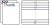
\includegraphics[width=\textwidth]{../intro-talk/figures/component-system}
\end{column}
\begin{column}{0.25\textwidth}
\centering
Syntax

\bigskip

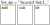
\includegraphics[width=\textwidth]{../intro-talk/figures/component-syntax}
\end{column}
\begin{column}{0.25\textwidth}
\centering
Semantics

\bigskip


\includegraphics[width=\textwidth]{../intro-talk/figures/component-semantics}
\end{column}
\end{columns}

\end{lrbox}

\begin{frame}{Model Components}
\usebox{\modelcomponentsbox}
\smash{}
\end{frame}

\subsection{System Description}

\begin{frame}{System Description}
\usebox{\modelcomponentsbox}
\smash{
	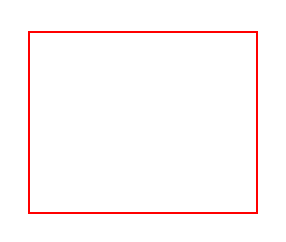
\begin{tikzpicture}[fill opacity=0.3]
		\draw[red,thick] (0, 0) rectangle (2.9, 2.3);
		\draw[draw=none] (0,0) rectangle (0, 2.35);
	\end{tikzpicture}
}
\end{frame}

\begin{frame}{System Description}

Three main components to system description:
\begin{itemize}
\item Register Files
\item Features
\item Instruction Sets
\end{itemize}

\end{frame}

\begin{frame}{Register File}

GenSim treats the register file as a set of flat memory regions (spaces)
with aliased `views'.

\end{frame}

\newsavebox{\codeboxone}
\begin{lrbox}{\codeboxone}
\begin{lstlisting}
ac_regspace(64) {
	bank RB (uint32, 0, 16, 4, 1, 4, 4);
	slot PC (uint32, 4, 60) PC;
	slot SP (uint32, 4, 52) SP;
}
\end{lstlisting}
\end{lrbox}

\newsavebox{\codeboxtwo}
\begin{lrbox}{\codeboxtwo}
\begin{lstlisting}
ac_regspace(256) {
	bank FP_SP (float,  0, 32, 4, 1, 4, 4);
	bank FP_DP (double, 0, 32, 8, 1, 8, 8);
	bank FP_Q (float, 0, 16, 16, 4, 4, 4);
}
\end{lstlisting}
\end{lrbox}

%\begin{frame}{Register File}

%Three types of entry
%\begin{itemize}
%\item Slot - single, non banked register
%\item Bank - `array' of values
%\item Vector Bank - `array' of vector values
%\end{itemize}

%\end{frame}

\begin{frame}[fragile]
\frametitle{Register File}

\centering
\only<1>{
	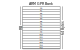
\includegraphics[height=0.5\textheight]{figures/regbank-rb}
}

\centering
\only<2>{
	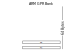
\includegraphics[height=0.5\textheight]{figures/regbank-slots}
}

\begin{minipage}[t]{0.95\textwidth}
\begin{block}{}
\usebox{\codeboxone}

\only<1>{
\smash{
	\begin{tikzpicture}[fill opacity=0.3]
		\draw[red,thick] (1.2, 1.05) rectangle (7.3, 1.35);
		\draw[draw=none] (0,0) rectangle (0, 2.35);
	\end{tikzpicture}
}}
\only<2>{
\smash{
	\begin{tikzpicture}[fill opacity=0.3]
		\draw[red,thick] (1.2, 0.35) rectangle (5.8, 1.05);
		\draw[draw=none] (0,0) rectangle (0, 2.35);
	\end{tikzpicture}
}}
\end{block}
\end{minipage}

\end{frame}

\begin{frame}{Register File - Vectors}

\only<1>{\centering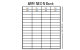
\includegraphics[height=0.5\textheight]{figures/regbank-fp}}
\only<2>{\centering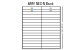
\includegraphics[height=0.5\textheight]{figures/regbank-fp-dp}}
\only<3>{\centering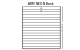
\includegraphics[height=0.5\textheight]{figures/regbank-fp-q}}

\begin{minipage}[t]{0.95\textwidth}
\begin{block}{}
\usebox{\codeboxtwo}

\only<1>{
\smash{
	\begin{tikzpicture}[fill opacity=0.3]
		\draw[red,thick] (1.2, 1.05) rectangle (7.8, 1.35);
		\draw[draw=none] (0,0) rectangle (0, 2.35);
	\end{tikzpicture}
}}
\only<2>{
\smash{
	\begin{tikzpicture}[fill opacity=0.3]
		\draw[red,thick] (1.2, 0.75) rectangle (7.8, 1.05);
		\draw[draw=none] (0,0) rectangle (0, 2.35);
	\end{tikzpicture}
}}
\only<3>{
\smash{
	\begin{tikzpicture}[fill opacity=0.3]
		\draw[red,thick] (1.2, 0.40) rectangle (7.8, 0.70);
		\draw[draw=none] (0,0) rectangle (0, 2.35);
	\end{tikzpicture}
}}
\end{block}
\end{minipage}

\end{frame}

\begin{frame}{Features}

Primarily performance feature - give hints to simulator about things 
which change infrequently.

\begin{itemize}
\item Actual processor features
\item FPU Enablement
\item Privilege mode
\item Configuration info
\end{itemize}

\end{frame}

\begin{frame}{Instruction Sets}

Which instruction sets are available to this architecture?
\begin{itemize}
\item Allows for instruction set switching
\item e.g. ARM $\Leftrightarrow$ Thumb\footnote{SAMOS'15: \url{https://doi.org/10.1109/SAMOS.2015.7363665}}
\end{itemize}

\end{frame}
